% !TEX TS-program = pdflatex
% !TEX encoding = UTF-8 Unicode

% This is a simple template for a LaTeX document using the "article" class.
% See "book", "report", "letter" for other types of document.

\documentclass[11pt]{article} % use larger type; default would be 10pt
\usepackage{wrapfig}
\usepackage{float}
\usepackage[utf8]{inputenc} % set input encoding (not needed with XeLaTeX)

%%% Examples of Article customizations
% These packages are optional, depending whether you want the features they provide.
% See the LaTeX Companion or other references for full information.

%%% PAGE DIMENSIONS
\usepackage{geometry} % to change the page dimensions
\geometry{a4paper} % or letterpaper (US) or a5paper or....
% \geometry{margin=2in} % for example, change the margins to 2 inches all round
% \geometry{landscape} % set up the page for landscape
%   read geometry.pdf for detailed page layout information

\usepackage{graphicx} % support the \includegraphics command and options

% \usepackage[parfill]{parskip} % Activate to begin paragraphs with an empty line rather than an indent

%%% PACKAGES
\usepackage{booktabs} % for much better looking tables
\usepackage{array} % for better arrays (eg matrices) in maths
\usepackage{paralist} % very flexible & customisable lists (eg. enumerate/itemize, etc.)
\usepackage{verbatim} % adds environment for commenting out blocks of text & for better verbatim
\usepackage{subfig} % make it possible to include more than one captioned figure/table in a single float
% These packages are all incorporated in the memoir class to one degree or another...

%%% HEADERS & FOOTERS
\usepackage{fancyhdr} % This should be set AFTER setting up the page geometry
\pagestyle{fancy} % options: empty , plain , fancy
\renewcommand{\headrulewidth}{0pt} % customise the layout...
\lhead{}\chead{}\rhead{}
\lfoot{}\cfoot{\thepage}\rfoot{}
\usepackage{graphicx}
\graphicspath{ {images/} }
%%% SECTION TITLE APPEARANCE
\usepackage{sectsty}
\allsectionsfont{\sffamily\mdseries\upshape} % (See the fntguide.pdf for font help)
% (This matches ConTeXt defaults)

%%% ToC (table of contents) APPEARANCE
\usepackage[nottoc,notlof,notlot]{tocbibind} % Put the bibliography in the ToC
\usepackage[titles,subfigure]{tocloft} % Alter the style of the Table of Contents
\renewcommand{\cftsecfont}{\rmfamily\mdseries\upshape}
\renewcommand{\cftsecpagefont}{\rmfamily\mdseries\upshape} % No bold!

%%% END Article customizations

%%% The "real" document content comes below...

\title{User Modelling Using NMF for Expedia Hotel Recommendation}
\author{Ronghao Yang\\ID: 20511820\\University of Waterloo}
%\date{} % Activate to display a given date or no date (if empty),
         % otherwise the current date is printed 

\begin{document}
\maketitle

\begin{abstract}

\end{abstract}
\section{Introduction}
Have you ever wondered, why can't you find the best music on Spotify? Or the most interesting book on Amazon? Or the finest hotel in the city of New York? In today's world, we want the service we get from the service providers (no matter online or offline) to be tailored to our interests, which means the services these days better to be personalized to amaze the customers. This is why recommendation systems are crucial in such business applications.\\

\section{Non-negative Matrix Factorization (NMF)}
\paragraph{• Introduction to NMF}\mbox{}\\
$NMF$ is a matrix factorization algorithm which factorize a big matrix $V$($m$ by $n$) into two smaller matrices $W$($m$ by $r$) and $H$($r$ by $n$). \\
\centerline{$V$ $\approx$ $W$ $\times$ $H$}\\
For each column $v_{i}$ in $V$, we have\\
\centerline{$v_{i}$ $\approx$ $W$ $\times$ $h_{i}$}\\
where $h_{i}$ is the corresponding column in $H$, in other words, every column in $V$ is a linear combination of $W$ where $H$ is the coefficient matrix. Geometrically, $NMF$ projects the data points in higher dimensional space to the lower dimensional space formed by the basis vectors in $W$, and $H$ contains the projected coefficients.\\
To integrate the theory with the context, matrices are commonly seen in recommendation problems, with columns and rows being users and the corresponding items. When $NMF$ factorizes such a matrix into $W$ and $H$, the columns in $W$ contains the hidden features of the original matrix. Each basis vector in $W$ can be viewed as basic user type, every user therefore is represented as a linear combination of such basic user typrs which are .\\
\centerline{$u$ = $a_1w_1+a_2w_2+....+a_rw_r$}
where $u$ is a single user and $a_is$ are the coefficients.
Besides, such user-item matrices are usually sparse (with high percentage of missing values), $NMF$ with EM algorithm can reconstruct the original matrix by filling out the missing values.\\

Here is an example of how $NMF$ works, the number of basis was set to be 100(which might not be optimal in this case):
\begin{figure}[!htb]
\minipage{0.25\textwidth}
  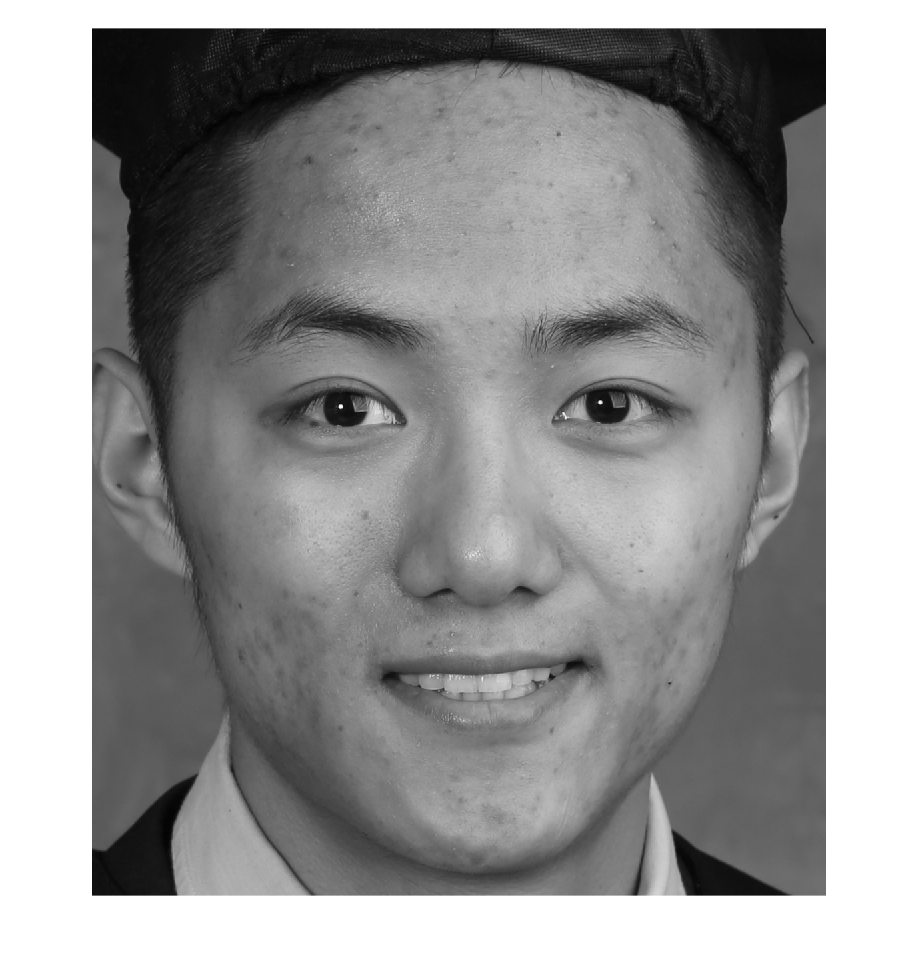
\includegraphics[width=\linewidth]{mySelfieOriginal.png}
  \caption{Original face image without any missing values}\label{fig:selfie1}
\endminipage\hfill
\minipage{0.25\textwidth}
  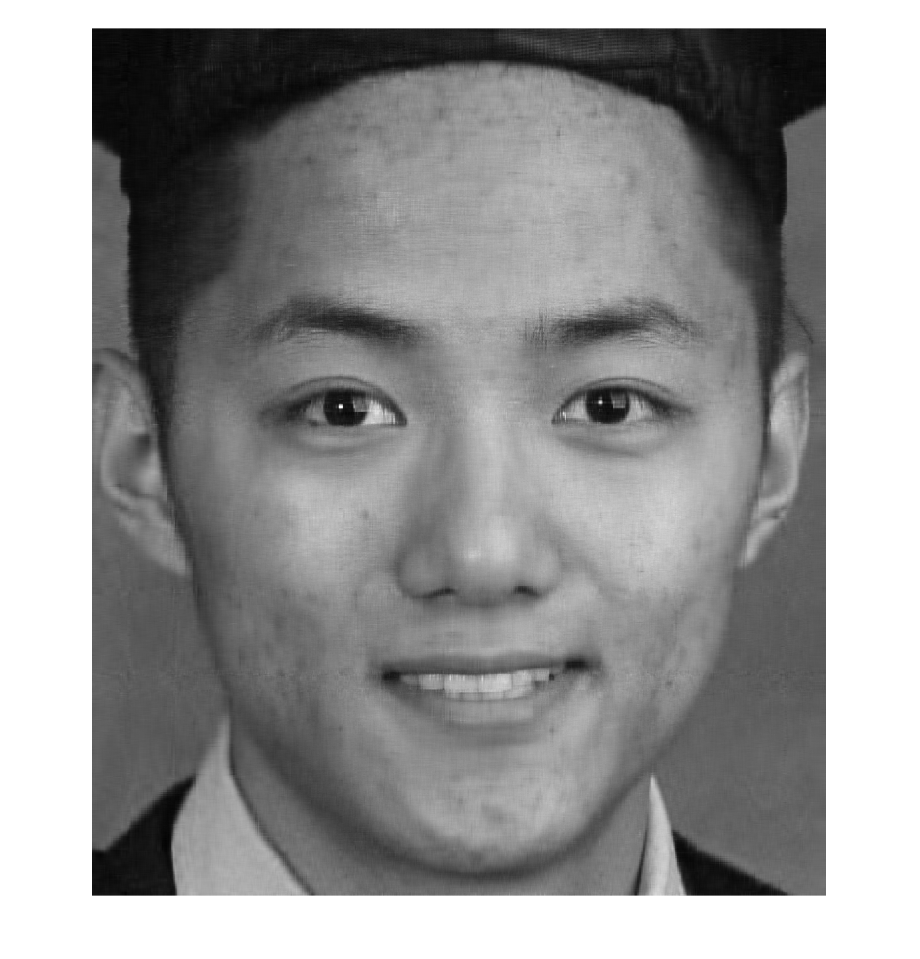
\includegraphics[width=\linewidth]{mySelfie50M100R.png}
  \caption{Face reconstruction with 50$\%$ missing values in the original image}\label{fig:selfie2}
\endminipage\hfill
\minipage{0.25\textwidth}%
  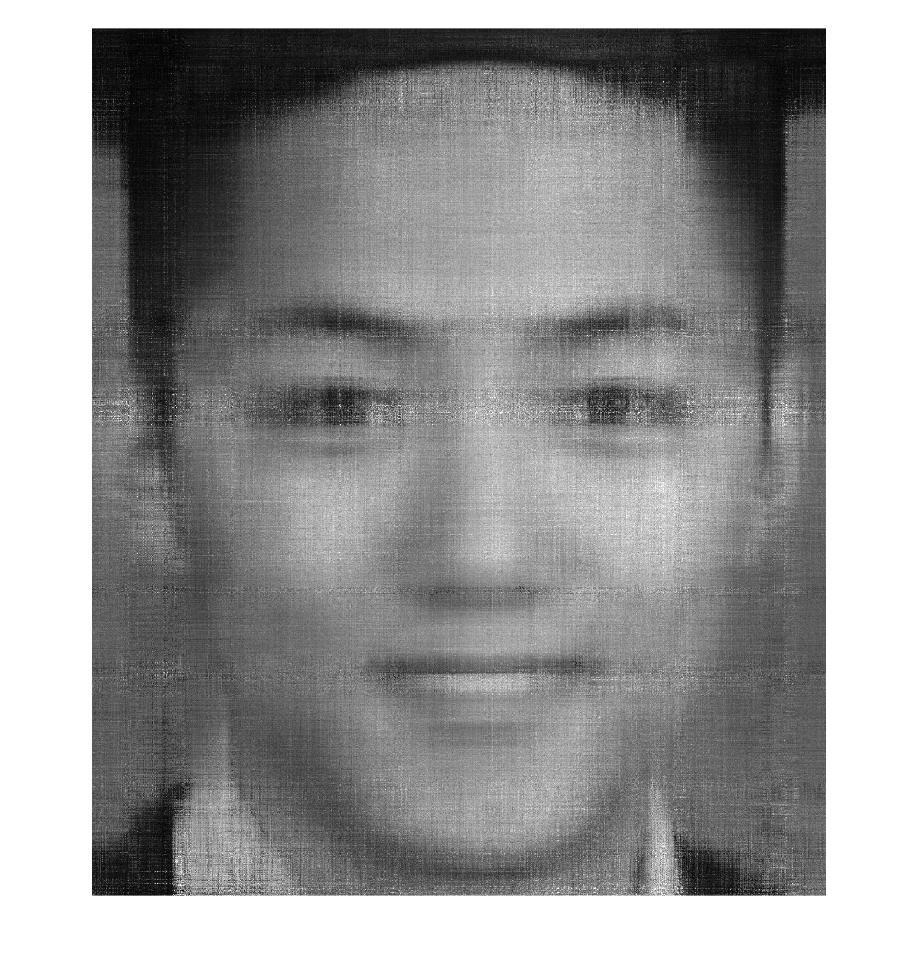
\includegraphics[width=\linewidth]{mySelfie90M100R.png}
  \caption{Face reconstruction with 90$\%$ missing values in the original image}\label{fig:siefie3}
\endminipage
\end{figure}
 

\paragraph{• Related work}\mbox{}\\
In 2014 Yu $\&$ Riedl from Georgia Tech have published a paper\cite{nmf1} about a recent success of $NMF$ for interactive narrative recommendation system. The research was to build a drama manager that learns a model of the player’s storytelling preferences and automatically recommends a narrative experience that is predicted to optimize the player’s experience while conforming to the human designer’s storytelling intentions \cite[p.~1]{nmf1}.\\
In their research, a new method called $Prefix-Based\;Collaborative\;Filtering$ (PBCF) \cite[p.~2]{nmf1} has been introduced in which each prefix is a sequence of story plots. Based on $PBCF$, a prefix-rating matrix was constructed in which each row represents a prefix, each column represents a player, every entry in the matrix is the numerical rating rated by a player for a prefix. Similar to most recommendation problems, this matrix is sparse, due to the nature that it is impossible for a single player to encounter all the prefixes.\\
$NMF$ was applied to this matrix to learn the player types
\begin{figure}[!htb]
\caption{Prefix rating matrix $\cite[p.~4]{nmf1}$}
\centering
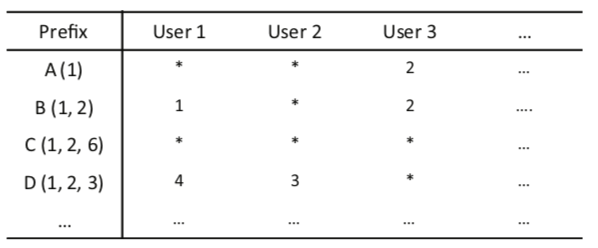
\includegraphics[width=0.5\textwidth]{prefixrating}
\end{figure}\\

\paragraph{• NMF algorithm}\mbox{}\\
In $Algorithms\;for\;Non-negative\;Matrix\; Factorization$ published by Daniel F. Lee and H. Sebastian Seung, several $NMF$ algorithms have been introduced. One of which is\\
\centerline{$H_{\alpha\mu}$ = $H_{\alpha\mu}\frac{(W^{T}R)_{\alpha\mu}}{(W^{T}WH)_{\alpha\mu}}$, $W_{i\alpha}$ = $W_{i\alpha}\frac{(RH^{T})_{i\alpha}}{(WHH^{T})_{i\alpha}}$ \cite[p.~3]{nmfalg}}\\
For predicting the new user 


\section{Experiment}
\subsection{Dataset}
The dataset we use for experiment is the Expedia hotel recommendation dataset from Kaggle competition in 2016. This dataset contains the hotel booking information of more than 2,000,000 users, of which the training set is obtained from 2013 and 2014 user data and the test set is obtained from 2015 user data.\\
In the data set, each column represent a user, each column contains the hotel booking information of the user. Such columns are date$\_$time. site$\_$name, posa$\_$continent, user$\_$location$\_$country, user$\_$location$\_$region, user$\_$location$\_$city, orig$\_$destination$\_$dista, user$\_$id, is$\_$mobile, is$\_$package, channel, srch$\_$ci, srch$\_$co, srch$\_$adults$\_$cnt, srch$\_$rm$\_$cnt, srch$\_$destination$\_$id, srch$\_$destination$\_$type$\_$id, hotel$\_$continent, hotel$\_$country, hotel$\_$market, is$\_$booking, cnt, and hotel$\_$cluster is what to be predicted. Moreover, for each hotel cluster, there are $149$ numerical latent descriptions.
\subsection{Modification on dataset}
Among all the columns, the date data is string data instead of numerical. The date in the testing set is one or two years later that the date in the training set, moreover, different user ids in this dataset may represent the same user. For the purpose of simplifying of the data set, I have removed the date coulumns. Then the user types will only be represented by numerical values.
\subsection{User modeling and Feature selection}
When using $NMF$ for building the user model, each basis user type is represented by the combination of different features. For example, assume we have $W$ as a user model which has 4 columns ($w_{1}, w_{2}, w_{3}, w_{4}$), $w_{1}$ represent users who love luxurious hotels, $w_{2}$ represent users who prefer cheaper hotels, $w_{3}$ represent users who want to live in downtown, $w_{4}$ represent users who dersire great hotel service. Then a new user maybe of 10\% of type 1, 30\% of type 2, 20\% of type 3 and 40\% of type 3.\\    
For feature selection, in some cases, we may also be able to select the number of basis based on some prior or domain knowledge. However, in our case, no proven knowledge is available. $NMF$ is capable of selecting the number basis user type by running cross validations. The number of basis that generates the smallest cross validation error is selected.\\
When running cross validation, $10-fold$ cross validation is selected. The loss metric is set to the rmse value between two matrices.\\\\
\centerline{$rmse_{A,B}$ = $\sqrt{avg_{ij}((A_{ij}-B_{ij})^{2})}$}

\paragraph{• Method 1}\mbox{}\\
For method 1, $KNN$ has been implemented as a complementary algorithm to $NMF$ for predicting the hotel clusters. In this method, we build the user model only using the general information of Expedia users without the latent description of search regions. Each user type is simply defined by user actions and other information in the training set, such as search location, is mobile, etc.\\
In the beginning of the training process, we apply $NMF$ on the training set to compute the user model $W$. Then we apply the computed model $W$ on the testing set to compute the coefficients($H$) of the testing users. Once we have the coefficients of a testing user, we go back to the training set and use $KNN$ to find what hotel cluster users that have the similar coefficients choose, then we use that hotel cluster as a prediction for the unknown user.

\begin{figure}[H] 
  \begin{minipage}[H]{0.5\linewidth}\label{ m1cv1} 
    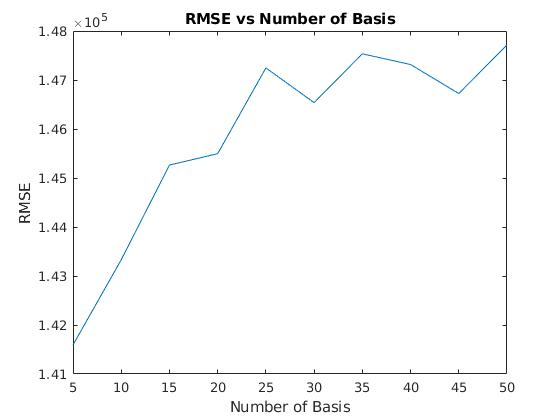
\includegraphics[width=1\linewidth]{m1CV1.jpg} 
    \caption{Cross validation with number of basis 5, 10, 15, .., 50} 
  \end{minipage} 
  \begin{minipage}[H]{0.5\linewidth}\label{ m1cv2} 
    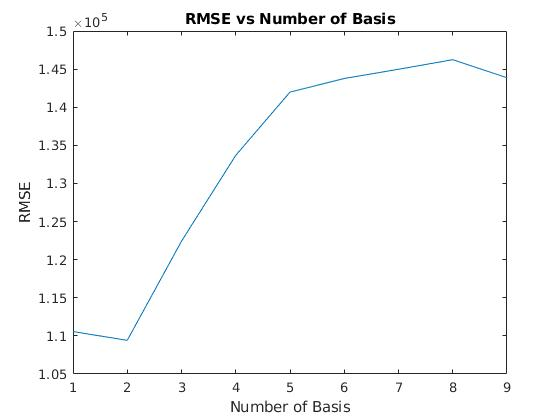
\includegraphics[width=1\linewidth]{m1CV2.jpg} 
    \caption{Cross validation with number of basis 1, 2, 3, ...9} 
  \end{minipage} 
  \begin{minipage}[H]{0.5\linewidth}\label{ m1nocv} 
    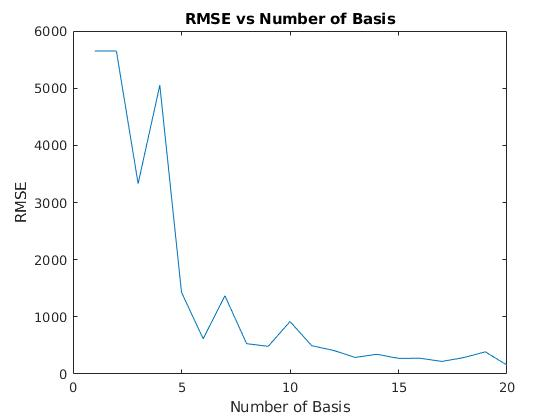
\includegraphics[width=1\linewidth]{m1NoCV.jpg} 
    \caption{Testing basis without using cross validation} 
  \end{minipage}
  \hfill
\end{figure}

\centerline{
\begin{tabular}[H]{ |p{1.5cm}||p{1.5cm}|p{1.5cm}|p{1.5cm}|p{1.5cm}|p{1.5cm} | }
 \hline
 \multicolumn{6}{|c|}{Results using method 1} \\
 \hline
& m=2 &m=5&m=10&m=15&m=20\\
 \hline
k = 1   & AF    &AFG&   004&005&hello\\
 \hline
k = 3  & AF    &AFG&   004&005&hello\\
 \hline
 k = 5   & AF    &AFG&   004&005&hello\\
 \hline
 k = 7  & AF    &AFG&   004&005&hello\\
 \hline
 k = 9   & AF    &AFG&   004&005&hello\\
 \hline
\end{tabular}
}

\paragraph{• Method 2}\mbox{}\\
For method 2, $KNN$ has also been implemented as a complementary algorithm to $NMF$ for predicting the hotel clusters. However, the exact method is different. In this method, the latent description of search regions has been used when building the user model. Compared to method 1, now each basis user type is also described by the latent variables.\\
In the beginning of the training process, we apply $NMF$ on the training set to compute the user model $W$. Then we use the computed model $W$ to computed the associated latent hotel descriptions of the user's potential hotel cluster. At the end, we apply $KNN$ algorithm on the computed latent hotel descriptions to compute the actual hotel cluster.
\begin{figure}[H] 
  \begin{minipage}[H]{0.5\linewidth}\label{ m1cv1} 
    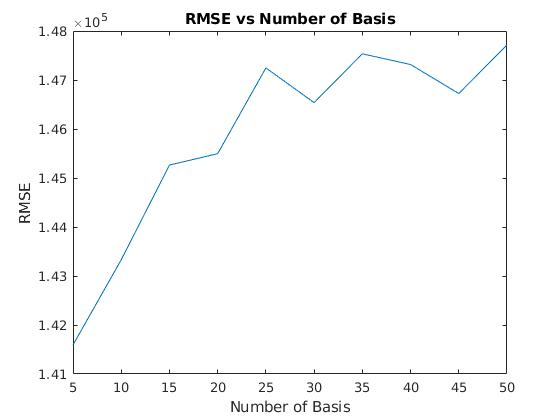
\includegraphics[width=1\linewidth]{m1CV1.jpg} 
    \caption{Cross validation with number of basis 5, 10, 15, .., 50} 
  \end{minipage} 
  \begin{minipage}[H]{0.5\linewidth}\label{ m1cv2} 
    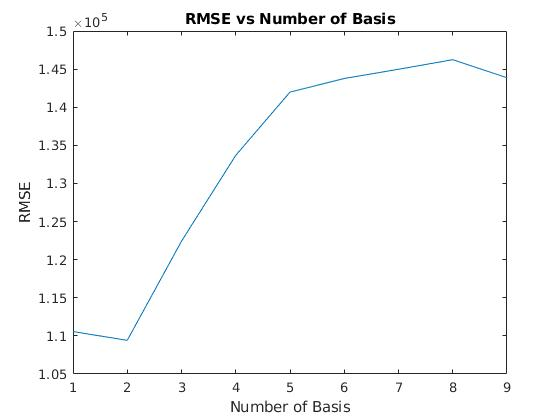
\includegraphics[width=1\linewidth]{m1CV2.jpg} 
    \caption{Cross validation with number of basis 1, 2, 3, ...9} 
  \end{minipage} 
  \begin{minipage}[H]{0.5\linewidth}\label{ m1nocv} 
    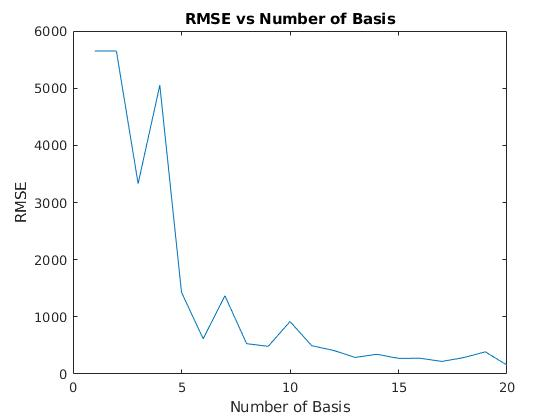
\includegraphics[width=1\linewidth]{m1NoCV.jpg} 
    \caption{Testing basis without using cross validation} 
  \end{minipage}
  \hfill
\end{figure}
\centerline{
\begin{tabular}[H]{ |p{1.5cm}||p{1.5cm}|p{1.5cm}|p{1.5cm}|p{1.5cm}|p{1.5cm} | }
 \hline
 \multicolumn{6}{|c|}{Results using method 1} \\
 \hline
& m=2 &m=5&m=10&m=15&m=20\\
 \hline
k = 1   & AF    &AFG&   004&005&hello\\
 \hline
k = 3  & AF    &AFG&   004&005&hello\\
 \hline
 k = 5   & AF    &AFG&   004&005&hello\\
 \hline
 k = 7  & AF    &AFG&   004&005&hello\\
 \hline
 k = 9   & AF    &AFG&   004&005&hello\\
 \hline
\end{tabular}
}
\subsection{Results}
\subsection{Comparision with other algorithms}
As in the papers and reports regarding the Expedia hotel recommendation competition, $NMF$ has never been implemented.
\section{Extra Experiment}


\section{Conclusion}


\section{Discussion}

\section{Note}
All the algorithms used for this project, including $NMF$, $KNN$ have been implemented by myself, no libraries have been used. Source code is available upon request.
\section{Acknowledgement}
I greatly acknowledge Dr.Yaoliang Yu for the amazing knowledge he shared with us and his support through out the term.


\begin{thebibliography}{9}
\bibitem{nmf1} 
Hong Yu and Mark O. Riedl.
\textit{Personalized Interactive Narratives via Sequential
Recommendation of Plot Points}
IEEE Transactions on Computational Intelligence and AI in Games, 6(2):174–187, 2014.

\bibitem{nmfalg} 
Daniel D. Lee and Seung, H. Sebastian.
\textit{Algorithms for Non-negative Matrix Factorization}
Advances in Neural Information Processing Systems 13, 556--562, 2001

\bibitem{expedia} 
Daniel D. Lee and Seung, H. Sebastian.
\textit{Algorithms for Non-negative Matrix Factorization}
Advances in Neural Information Processing Systems 13, 556--562, 2001

\end{thebibliography}

\end{document}
